\chapter{Example Chapter}
\label{chap:example}

Here is a link to the {\textit{Section~\ref{sec:example.examplesec}}}. There is also this very fine figure {\textit{Figure~\ref{fig:example.c}}}. I also want to draw your attention to the information in this footnote.\footnote{Footnotes are like bicycles - there is always room for n+1} Of course we must also consider \cite{leach2018iain} and \cite{martin2021shadow}.

\lipsum[1]

\section{Example Section}
\label{sec:example.examplesec}

\lipsum[2]

\begin{figure}[h!]
	\centering
	\captionsetup{justification=centering}
	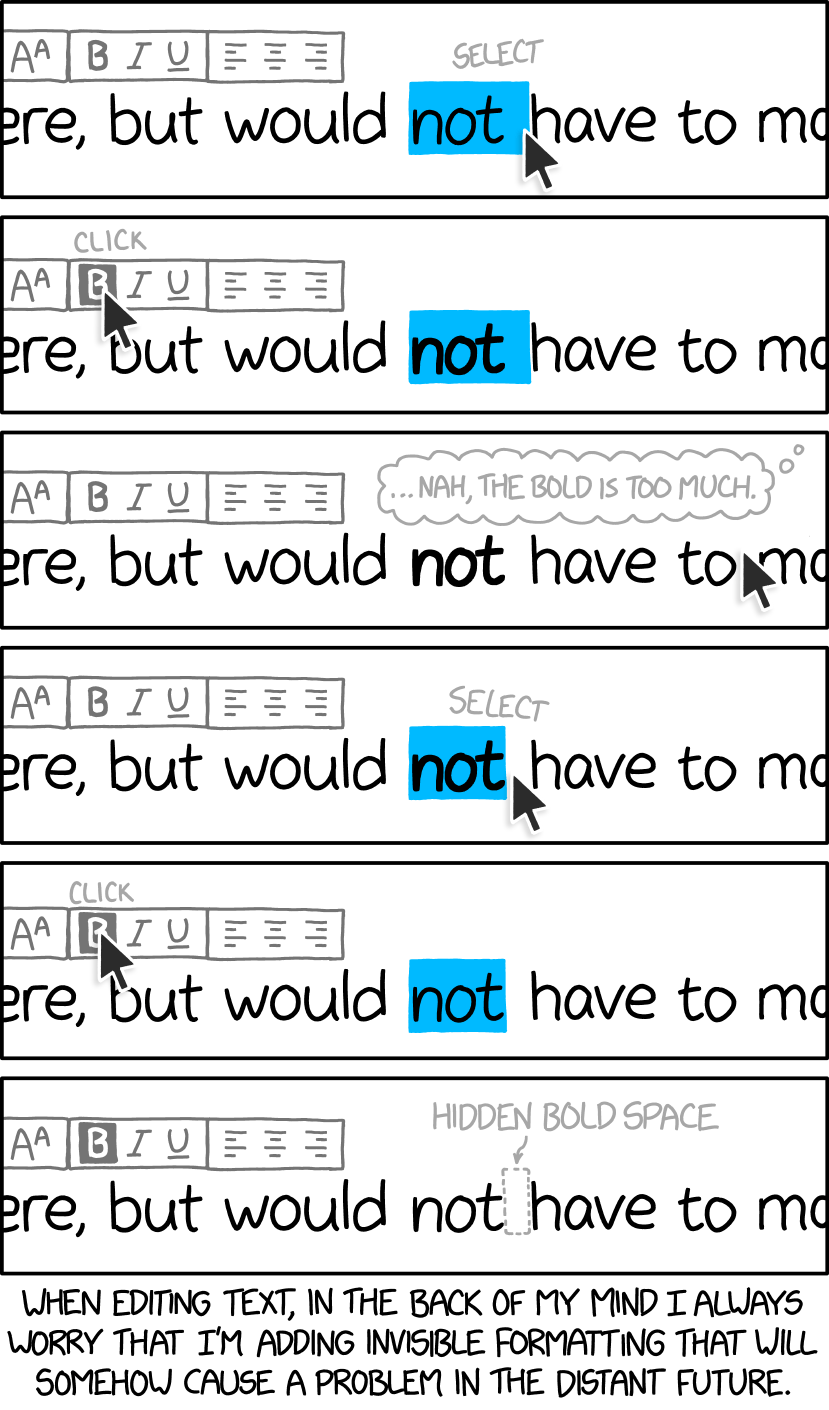
\includegraphics[height=8cm]{images/examples/xkcd_2109_invisible_formatting_2x.png}
	\caption[Example figure A]{Example figure that should probably be removed at some point\protect\footnotemark}
	\label{fig:example.a}
\end{figure}
\footnotetext{Attribution: xkcd 1205 (\url{https://xkcd.com/1205})}


\section{Another Section}
\label{sec:example.another}

\newpage

\lipsum[3]

\begin{figure}[h!]
	\centering
	\captionsetup{justification=centering}
	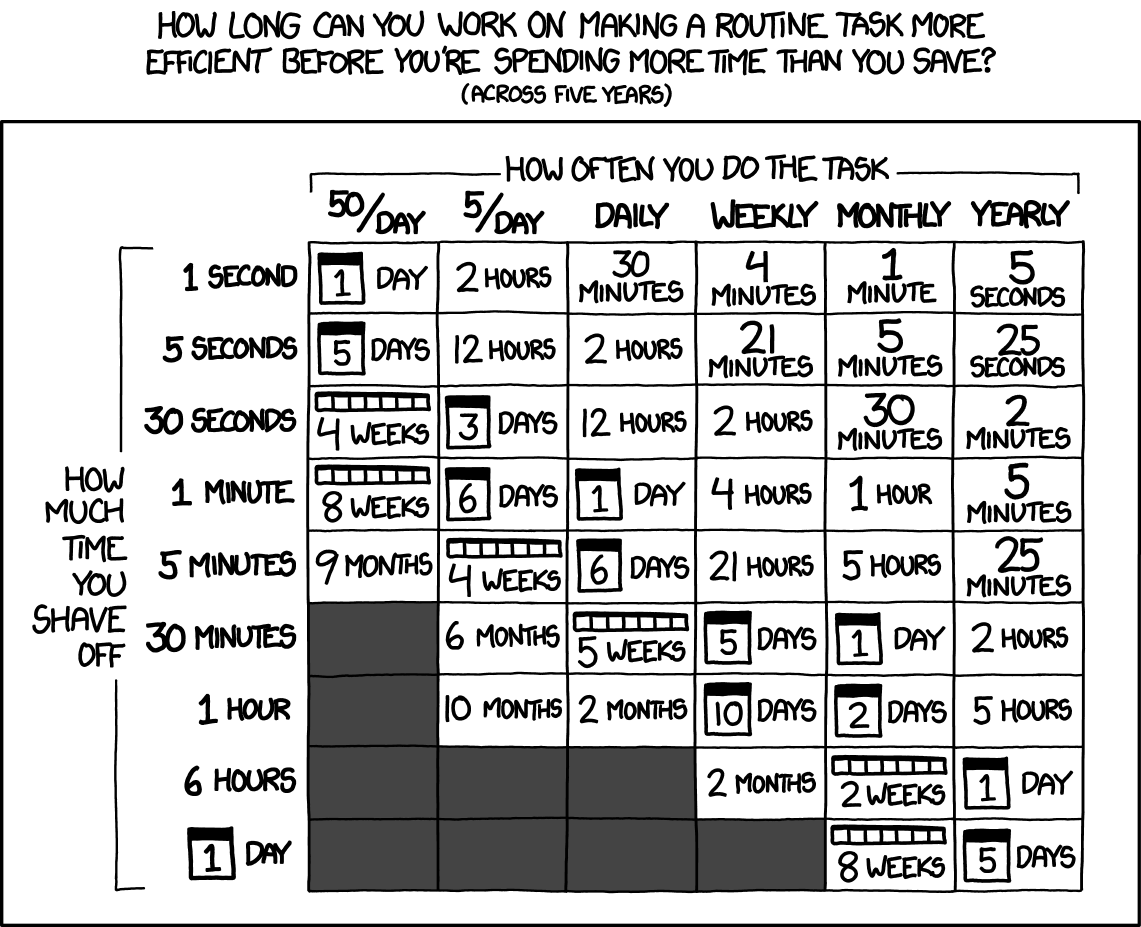
\includegraphics[height=8cm]{images/examples/xkcd_1205_is_it_worth_the_time_2x.png}
	\caption[Example figure B]{I feel this table is relevant to many aspects of PhD work\protect\footnotemark}
	\label{fig:example.b}
\end{figure}
\footnotetext{Attribution: xkcd 2109 (\url{https://xkcd.com/2109})}

\lipsum[4]

\begin{figure}[h!]
	\centering
	\captionsetup{justification=centering}
	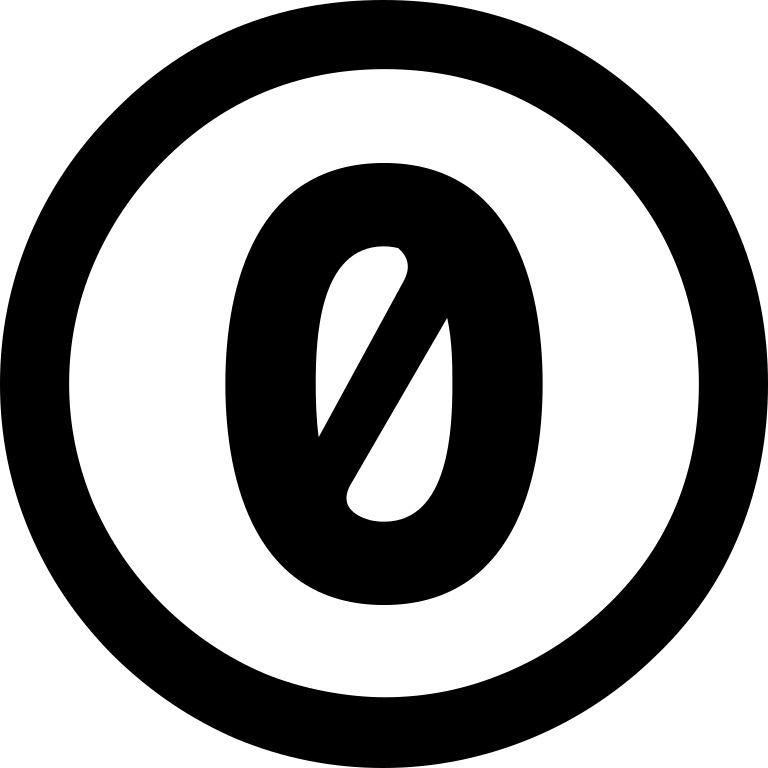
\includegraphics[height=5cm]{images/examples/cc-zero.png}
	\caption{Example figure with no attribution}
	\label{fig:example.c}
\end{figure}


\subsection{Foo}
\label{subsec:example.another_foo}

\lipsum[5-6]


\subsection{Bar}
\label{subsec:example.another_bar}

\begin{table}[h]
	\small{
		\centering
		{%
			\scalebox{0.86}{
				{\begin{tabular}{|p{5.5cm}|>{\centering\arraybackslash}p{2cm}|p{11cm}|}
						\hline
						\rowcolor[HTML]{EFEFEF} 
						{\color[HTML]{000000} \textbf{Some important numbers}} & {\color[HTML]{000000} \textbf{Frequency}} & {\color[HTML]{000000} \textbf{Category}} \\ \hline
						\rowcolor[HTML]{FFFFFF} 
						1 (Strongly disagree) & 1 & Some text here \\ \hline
						\rowcolor[HTML]{FFFFFF} 
						2 (Disagree) & 0 &  \\ \hline
						\rowcolor[HTML]{33FFFF} 
						3 (Dunno) & 2 & Important stuff \\ \hline
						\rowcolor[HTML]{FFFFFF} 
						4 (Agree) & 12 & Blah  \\ \hline
						\rowcolor[HTML]{FFFFFF} 
						5 (Strongly agree) & 9 & Yes  \\ \hline
					\end{tabular}%
	}}}}
	\caption{\textit{Some important numbers}}
	\label{tab:example.a}
\end{table}

\begin{theorem}[Pythagorean theorem]
	\label{the:example.pythagorean}
	This is a theorem about right triangles and can be summarised in the next 
	equation: 
	\[ x^2 + y^2 = z^2 \]
\end{theorem}

And a consequence of theorem \ref{the:pythagorean} is the statement in the next 
corollary.

\begin{corollary}
	There's no right rectangle whose sides measure 3cm, 4cm, and 6cm.
\end{corollary}

\begin{lemma}
	Given two line segments whose lengths are \(a\) and \(b\) respectively there is a 
	real number \(r\) such that \(b=ra\).
\end{lemma}

\lipsum[7]

